\section{Tuần 5: Biến đổi Màu sắc -- Ánh xạ Mức xám Tuyến tính, Phi tuyến và dựa trên Hàm Mật độ Xác suất}
\label{sec:week5}

Các câu hỏi trong tuần này dựa trên Bài giảng số 3 (\emph{Image Pre-processing -- 3.1. Color Transformations})~\citep{xlav_lec3}. Toàn bộ các phép biến đổi trong tuần đều là \emph{phép toán điểm} (point operation): giá trị mới tại $(x, y)$ chỉ phụ thuộc vào giá trị cũ tại chính $(x, y)$,
\begin{equation}
g(x, y) = T\big(f(x, y)\big),
\label{eq:w5_point_op}
\end{equation}
trong đó $f$ là ảnh vào, $g$ là ảnh ra, $T: \{0, \ldots, n_G - 1\} \rightarrow \{0, \ldots, n_G - 1\}$ là hàm ánh xạ mức xám và $n_G$ là số mức xám ($n_G = 256$ với ảnh 8 bit). Vì $T$ chỉ có $n_G$ giá trị đầu vào, mọi phép biến đổi trong tuần đều cài đặt được bằng một \emph{bảng tra} (lookup table, LUT) $n_G$ phần tử, với chi phí $O(n_G + NM)$ cho ảnh $N \times M$.

% =====================================================================
\subsection{Biểu thức \texorpdfstring{$g = a \cdot f$}{g = a f} và sự thay đổi độ tương phản}
\label{subsec:w5_contrast}

\textit{Câu hỏi: Bài giảng định nghĩa phép thay đổi độ tương phản (contrast modification) bởi biểu thức $g(x, y) = a \cdot f(x, y)$~\citep{xlav_lec3}. Hãy giải thích vì sao biểu thức này làm thay đổi được độ tương phản của ảnh. Với giá trị nào của $a$ thì độ tương phản tăng, với giá trị nào thì độ tương phản giảm?}

\textbf{Độ tương phản là gì.} Độ tương phản đo \emph{mức chênh lệch} độ sáng giữa các vùng trong ảnh. Hai cách định lượng thường dùng là chênh lệch giữa hai điểm ảnh $|f(p) - f(q)|$ (hoặc khoảng động $f_{\max} - f_{\min}$) và độ lệch chuẩn của mức xám $\sigma_f$ (độ tương phản RMS)~\citep{gonzalez2018digital}. Mắt người phân biệt hai vùng được hay không là nhờ chênh lệch này, không phải nhờ giá trị tuyệt đối của từng vùng.

\textbf{Tác động của $a$.} Với hai điểm ảnh bất kỳ $p$, $q$:
\begin{equation}
g(p) - g(q) = a\,\big(f(p) - f(q)\big), \qquad \sigma_g = |a|\,\sigma_f, \qquad g_{\max} - g_{\min} = |a|\,(f_{\max} - f_{\min}).
\label{eq:w5_contrast_scale}
\end{equation}
Mọi chênh lệch mức xám đều được nhân với cùng hệ số $|a|$, vì vậy $a$ điều khiển trực tiếp độ tương phản. Nói cách khác, $a$ là \emph{hệ số góc} của đường thẳng ánh xạ: một khoảng mức xám rộng $\Delta f$ ở đầu vào được ánh xạ thành khoảng rộng $\Delta g = |a|\,\Delta f$ ở đầu ra.
\begin{itemize}
    \item $a > 1$: các mức xám bị \emph{giãn} ra, chênh lệch lớn hơn $\Rightarrow$ \textbf{tăng} độ tương phản. Ví dụ ảnh có $f \in [60, 120]$, với $a = 1{,}5$ thì $g \in [90, 180]$: khoảng động tăng từ $60$ lên $90$.
    \item $0 < a < 1$: các mức xám bị \emph{nén} lại $\Rightarrow$ \textbf{giảm} độ tương phản. Với $a = 0{,}5$, ảnh trên trở thành $g \in [30, 60]$, khoảng động chỉ còn $30$.
    \item $a = 1$: ảnh không đổi. $a = 0$: ảnh đen hoàn toàn, mất toàn bộ thông tin.
    \item $a < 0$: thứ tự sáng -- tối bị đảo ngược (ảnh âm bản); độ lớn tương phản là $|a|$ lần nhưng cần thêm hằng số $b$ để kết quả nằm trong miền hợp lệ, ví dụ ảnh âm bản $g = -f + (n_G - 1)$.
\end{itemize}

\textbf{Lưu ý khi cài đặt.} (i) \emph{Bão hòa}: với $a > 1$, mọi điểm có $f > (n_G - 1)/a$ bị cắt về $n_G - 1$. Ví dụ $a = 2{,}5$ thì mọi điểm $f \ge 102$ đều thành $255$, chi tiết vùng sáng mất vĩnh viễn. (ii) \emph{Lượng tử hóa}: với $a > 1$, các mức xám nguyên liên tiếp được đưa ra xa nhau, giữa chúng xuất hiện ``khoảng trống'' trên lược đồ, ảnh có thể bị phân dải (banding); với $a < 1$, nhiều mức xám bị gộp thành một sau khi làm tròn, không khôi phục được. (iii) Phép nhân $a \cdot f$ \emph{đồng thời} làm thay đổi độ sáng trung bình ($\bar g = a \bar f$). Muốn chỉ thay đổi độ tương phản mà giữ nguyên độ sáng trung bình, ta lấy giá trị trung bình $\bar f$ (hoặc mức giữa $128$) làm tâm co giãn:
\begin{equation}
g(x, y) = a\,\big(f(x, y) - \bar f\big) + \bar f,
\end{equation}
đây chính là dạng $g = a f + b$ với $b = (1 - a)\bar f$ của mục \emph{Brightness + Contrast modification} trong bài giảng.

% =====================================================================
\subsection{Tăng kích thước tập dữ liệu ảnh từ 1.000 lên 5.000 ảnh}
\label{subsec:w5_augmentation}

\textit{Câu hỏi: Giả sử ta có một tập dữ liệu gồm $1.000$ ảnh và muốn tăng lên $5.000$ ảnh (ví dụ để huấn luyện một mô hình học máy). Cần làm gì?}

Khi không thể thu thập và gán nhãn thêm dữ liệu thật, ta dùng \textbf{tăng cường dữ liệu} (data augmentation): sinh ra ảnh mới từ ảnh có sẵn bằng các phép biến đổi \emph{không làm thay đổi nhãn}~\citep{shorten2019survey}. Với mỗi ảnh gốc, sinh thêm $4$ phiên bản biến đổi ngẫu nhiên sẽ được $1.000 \times (1 + 4) = 5.000$ ảnh. Các nhóm phép biến đổi:

\begin{enumerate}
    \item \textbf{Biến đổi màu sắc (photometric)} — chính là nội dung của tuần này: thay đổi độ sáng $g = f + b$, độ tương phản $g = a f$ (Mục~\ref{subsec:w5_contrast}), ánh xạ phi tuyến (log, mũ, gamma), cân bằng lược đồ, CLAHE; với ảnh màu có thể thay đổi ngẫu nhiên $H$, $S$, $V$ (color jitter). Các phép này mô phỏng sự khác nhau về điều kiện chiếu sáng và thiết bị chụp.
    \item \textbf{Biến đổi hình học}: lật ngang, xoay, co giãn, cắt ngẫu nhiên, tịnh tiến, biến đổi affine/phối cảnh. Các phép này cần nội suy mức xám (Mục~\ref{subsec:w6_augment_interp}), mô phỏng sự thay đổi vị trí, góc nhìn và khoảng cách tới vật.
    \item \textbf{Suy giảm chất lượng}: thêm nhiễu (Mục~\ref{subsec:w6_noise_func}), làm mờ, nén JPEG, giảm độ phân giải — giúp mô hình bền vững với ảnh kém chất lượng.
    \item \textbf{Che khuất và trộn ảnh}: xóa ngẫu nhiên một vùng (Cutout/Random Erasing), trộn hai ảnh và nhãn của chúng theo tỉ lệ $\lambda$ (mixup)~\citep{zhang2018mixup}, dán một mảng ảnh này lên ảnh khác (CutMix)~\citep{yun2019cutmix}.
    \item \textbf{Tổng hợp ảnh}: sinh ảnh mới bằng mô hình tạo sinh (GAN, mô hình khuếch tán) hoặc dựng ảnh từ mô hình 3D; dùng khi các phép biến đổi đơn giản không tạo đủ sự đa dạng.
\end{enumerate}

\textbf{Các nguyên tắc cần tuân thủ.}
\begin{itemize}
    \item \emph{Bảo toàn nhãn}: phép biến đổi phải phù hợp với bài toán. Lật ngang ảnh chữ số ``6'' hay biển báo rẽ trái làm sai nhãn; đổi màu mạnh sẽ hỏng bài toán phân loại quả chín/xanh. Với bài toán phát hiện, phân đoạn, phải biến đổi cả hộp bao/mặt nạ cùng với ảnh.
    \item \emph{Chia tập trước khi tăng cường}: tách tập huấn luyện/kiểm thử trên $1.000$ ảnh gốc rồi mới tăng cường tập huấn luyện. Nếu tăng cường trước, các bản sao của cùng một ảnh nằm ở cả hai tập, kết quả đánh giá sẽ cao giả tạo.
    \item \emph{Tăng cường trực tuyến} (sinh ngẫu nhiên tại mỗi vòng huấn luyện) thường tốt hơn lưu cố định $5.000$ ảnh: mô hình thấy một biến thể mới ở mỗi vòng mà không tốn bộ nhớ.
    \item Ảnh tăng cường \emph{không chứa thông tin mới} về đối tượng, chỉ mã hóa các bất biến mà ta biết trước; vì vậy $5.000$ ảnh tăng cường vẫn kém $5.000$ ảnh thật.
\end{itemize}

% =====================================================================
\subsection{Ứng dụng của phép chuyển đổi mức xám}
\label{subsec:w5_applications}

\textit{Câu hỏi: Phép chuyển các mức xám của một ảnh sang các mức xám khác (ánh xạ mức xám) được dùng để làm gì? Nêu các ứng dụng.}

Mục đích chung là \emph{phân bố lại} các mức xám để thông tin cần quan tâm được thể hiện rõ hơn, hoặc để các ảnh khác nhau trở nên so sánh được với nhau. Các ứng dụng cụ thể:
\begin{enumerate}
    \item \textbf{Tăng cường ảnh để quan sát}: ảnh chụp thiếu sáng, thừa sáng, ngược sáng hoặc có độ tương phản thấp (trời mù, ảnh X-quang) được kéo giãn để mắt người thấy được chi tiết (ví dụ các ảnh ở trang 11--12 và 19--22 của bài giảng~\citep{xlav_lec3}).
    \item \textbf{Nén khoảng động}: ảnh có khoảng giá trị rất rộng (phổ Fourier, ảnh HDR, ảnh thiên văn, ảnh nhiệt) không hiển thị được trên màn hình 8 bit; phép log nén khoảng động này mà vẫn giữ chi tiết ở vùng giá trị nhỏ.
    \item \textbf{Cửa sổ hóa (windowing) trong ảnh y khoa}: ảnh CT có giá trị từ khoảng $-1000$ đến $+3000$ HU. Bác sĩ chọn một ``cửa sổ'' $[f_1, f_2]$ (cửa sổ phổi, cửa sổ xương, cửa sổ mô mềm) và ánh xạ tuyến tính lên $[0, 255]$ (Mục~\ref{subsec:w5_range_map}).
    \item \textbf{Chuẩn hóa trước khi phân tích}: đưa ảnh chụp trong các điều kiện ánh sáng khác nhau về cùng một phân bố mức xám (cân bằng hoặc đặc tả lược đồ), giúp các bước phân ngưỡng, so khớp mẫu, nhận dạng khuôn mặt, truy vấn ảnh ổn định hơn.
    \item \textbf{Tiền xử lý cho phân đoạn}: kéo giãn khoảng mức xám của đối tượng để tách đối tượng khỏi nền dễ hơn; trường hợp cực đoan là phân ngưỡng — một ánh xạ mức xám thành $2$ mức.
    \item \textbf{Hiệu chỉnh thiết bị}: hiệu chỉnh gamma để bù đặc tuyến phi tuyến của màn hình hoặc cảm biến; giảm số bit (lượng tử hóa lại) để lưu trữ hay hiển thị.
    \item \textbf{Hiệu ứng và tăng cường dữ liệu}: tạo ảnh âm bản, chỉnh màu trong các phần mềm biên tập; sinh thêm ảnh huấn luyện có độ sáng, độ tương phản khác nhau (Mục~\ref{subsec:w5_augmentation}).
\end{enumerate}

% =====================================================================
\subsection{Công thức ánh xạ khoảng mức xám \texorpdfstring{$[f_1, f_2]$}{[f1, f2]} sang \texorpdfstring{$[g_1, g_2]$}{[g1, g2]}}
\label{subsec:w5_range_map}

\textit{Câu hỏi: Bài giảng (trang 10) yêu cầu ánh xạ ảnh từ khoảng mức xám $[f_1, f_2]$ sang khoảng mức xám $[g_1, g_2]$~\citep{xlav_lec3}. Hãy thiết lập công thức của phép biến đổi này.}

Ta tìm phép biến đổi tuyến tính $g = a f + b$ thỏa $f_1 \mapsto g_1$ và $f_2 \mapsto g_2$, tức đường thẳng đi qua hai điểm $(f_1, g_1)$ và $(f_2, g_2)$:
\begin{equation}
\begin{cases} a f_1 + b = g_1 \\ a f_2 + b = g_2 \end{cases}
\;\Rightarrow\;
a = \frac{g_2 - g_1}{f_2 - f_1}, \qquad b = g_1 - a f_1 = \frac{g_1 f_2 - g_2 f_1}{f_2 - f_1} \quad (f_1 \ne f_2).
\end{equation}
Vậy
\begin{equation}
g(x, y) = \frac{g_2 - g_1}{f_2 - f_1}\,\big(f(x, y) - f_1\big) + g_1.
\label{eq:w5_range_map}
\end{equation}
Phép biến đổi giữ nguyên \emph{vị trí tương đối}: điểm nằm ở $t\%$ của $[f_1, f_2]$ sẽ nằm ở $t\%$ của $[g_1, g_2]$, vì $\frac{g - g_1}{g_2 - g_1} = \frac{f - f_1}{f_2 - f_1}$. Hệ số góc $a$ cho biết độ tương phản tăng ($g_2 - g_1 > f_2 - f_1$) hay giảm.

\textbf{Các điểm nằm ngoài $[f_1, f_2]$.} Nếu ảnh có điểm ảnh nằm ngoài khoảng $[f_1, f_2]$, cần quy ước thêm. Cách thường dùng là cắt ngưỡng (ánh xạ tuyến tính từng đoạn):
\begin{equation}
g = \begin{cases}
g_1, & f < f_1, \\
\dfrac{g_2 - g_1}{f_2 - f_1}(f - f_1) + g_1, & f_1 \le f \le f_2, \\
g_2, & f > f_2,
\end{cases}
\end{equation}
sau đó làm tròn về số nguyên. Cách khác là dùng ánh xạ ba đoạn, nối $[0, f_1] \to [0, g_1]$ và $[f_2, n_G - 1] \to [g_2, n_G - 1]$, để không mất thông tin ở hai đầu.

\textbf{Trường hợp đặc biệt.} Với $[f_1, f_2] = [f_{\min}, f_{\max}]$ của ảnh và $[g_1, g_2] = [0, 255]$, ta có phép \emph{kéo giãn độ tương phản} (contrast stretching), tận dụng toàn bộ khoảng động của thiết bị hiển thị. Vì $f_{\min}$, $f_{\max}$ rất nhạy với một vài điểm nhiễu, trong thực tế thường dùng phân vị $1\%$ và $99\%$ thay cho giá trị nhỏ nhất và lớn nhất. Ví dụ: $[f_1, f_2] = [50, 150]$, $[g_1, g_2] = [0, 255]$ cho $a = 2{,}55$, $b = -127{,}5$; điểm $f = 100$ (giữa khoảng) được ánh xạ thành $g = 127{,}5 \approx 128$ (giữa khoảng mới).

% =====================================================================
\subsection{Vì sao \texorpdfstring{$g = a f + b$}{g = af + b} được gọi là phép biến đổi tuyến tính}
\label{subsec:w5_why_linear}

\textit{Câu hỏi: Vì sao phép biến đổi $g = a f + b$ được gọi là phép biến đổi tuyến tính (linear mapping)?}

\textbf{Theo nghĩa đại số chặt chẽ, $T(f) = a f + b$ với $b \ne 0$ không phải là ánh xạ tuyến tính} mà là ánh xạ \emph{affine}. Ánh xạ tuyến tính phải thỏa tính cộng tính và tính thuần nhất, $T(u + v) = T(u) + T(v)$ và $T(\lambda u) = \lambda T(u)$, trong khi
\begin{equation}
T(u + v) = a(u + v) + b \ne (a u + b) + (a v + b) = T(u) + T(v) \quad \text{khi } b \ne 0,
\end{equation}
và $T(0) = b \ne 0$. Chỉ phép thay đổi độ tương phản $g = a f$ ($b = 0$) là tuyến tính theo nghĩa này.

Trong xử lý ảnh, tên gọi ``ánh xạ tuyến tính'' được dùng theo các nghĩa sau, và đều đúng:
\begin{enumerate}
    \item \textbf{Đồ thị là đường thẳng}: $g$ là đa thức bậc nhất theo $f$, phân biệt với các ánh xạ phi tuyến bậc cao hơn hoặc siêu việt (log, mũ) ở Mục 3.1.2 của bài giảng.
    \item \textbf{Hệ số góc không đổi}: $\frac{dg}{df} = a$ tại mọi mức xám. Mọi khoảng mức xám có cùng độ rộng $\Delta f$, \emph{dù nằm ở vùng tối hay vùng sáng}, đều được ánh xạ thành khoảng có cùng độ rộng $|a|\,\Delta f$: phép biến đổi tác động \emph{đồng đều} lên toàn bộ thang xám. Đây chính là điểm khác biệt cơ bản với ánh xạ log, mũ (Mục~\ref{subsec:w5_log_exp_proof}).
    \item \textbf{Tuyến tính trong tọa độ thuần nhất}: viết mức xám dưới dạng vector $(f, 1)^T$ thì
    $\begin{pmatrix} g \\ 1 \end{pmatrix} = \begin{pmatrix} a & b \\ 0 & 1 \end{pmatrix}\begin{pmatrix} f \\ 1 \end{pmatrix}$
    là phép nhân ma trận, tức một ánh xạ tuyến tính — cùng thủ thuật dùng cho phép tịnh tiến trong đồ họa máy tính. Nhờ đó, ghép nhiều phép biến đổi dạng $a f + b$ vẫn cho một phép biến đổi cùng dạng.
    \item \textbf{Bảo toàn tổ hợp lồi}: $T\big(\lambda u + (1 - \lambda) v\big) = \lambda T(u) + (1 - \lambda) T(v)$ với mọi $\lambda$. Vì vậy trung bình cộng của ảnh, phép nội suy và vị trí tương đối của các mức xám được bảo toàn: $\bar g = a \bar f + b$, $\sigma_g = |a|\sigma_f$, và hình dạng lược đồ không đổi, chỉ bị dịch chuyển và co giãn.
\end{enumerate}

% =====================================================================
\subsection{Chứng minh tính co giãn của ánh xạ logarit và ánh xạ mũ bằng đạo hàm}
\label{subsec:w5_log_exp_proof}

\textit{Câu hỏi: Trang 15 của bài giảng minh họa đồ thị hàm ánh xạ logarit $g(x, y) = c \log f(x, y)$ cùng hai khoảng mức xám đầu vào $\Delta f_1$, $\Delta f_2$ có độ rộng bằng nhau nhưng ở hai vị trí khác nhau trên trục $f$ ($\Delta f_1$ ở vùng tối, $\Delta f_2$ ở vùng sáng), cho ra hai khoảng đầu ra $\Delta g_1 > \Delta g_2$~\citep{xlav_lec3}. Sử dụng đạo hàm, hãy chứng minh rằng các khoảng đầu vào bằng nhau ở những vị trí khác nhau sẽ được hàm $c \log f$ co giãn khác nhau tương ứng với vị trí. Chứng minh tương tự cho hàm ánh xạ mũ $g(x, y) = e^{f(x, y)}$ (trang 18).}

\textbf{Ánh xạ logarit.} Xét $g(f) = c \ln f$ với $c > 0$, $f > 0$ (dùng logarit cơ số khác chỉ làm thay đổi hằng số $c$). Đạo hàm
\begin{equation}
g'(f) = \frac{c}{f} > 0, \qquad g''(f) = -\frac{c}{f^2} < 0.
\end{equation}
Vậy $g$ đồng biến (giữ thứ tự sáng -- tối) và $g'$ giảm dần theo $f$ ($g$ lõm). Xét khoảng $[f, f + \Delta]$ với $\Delta > 0$ cố định. Theo định lý giá trị trung bình Lagrange, tồn tại $\xi \in (f, f + \Delta)$ sao cho
\begin{equation}
\Delta g(f) = g(f + \Delta) - g(f) = g'(\xi)\,\Delta = \frac{c}{\xi}\,\Delta.
\end{equation}
Chặt chẽ hơn, $\Delta g(f) = \int_f^{f + \Delta} \frac{c}{t}\,dt = c \ln\!\left(1 + \frac{\Delta}{f}\right)$ và
\begin{equation}
\frac{d}{df}\,\Delta g(f) = g'(f + \Delta) - g'(f) = \frac{c}{f + \Delta} - \frac{c}{f} = -\frac{c\,\Delta}{f(f + \Delta)} < 0.
\end{equation}
Do đó $\Delta g(f)$ là hàm \textbf{giảm ngặt} theo vị trí $f$ của khoảng: với $\Delta f_1 = \Delta f_2 = \Delta$ và $\Delta f_1$ nằm bên trái $\Delta f_2$ (vùng tối hơn), ta luôn có $\Delta g_1 > \Delta g_2$. Đó chính là điều cần chứng minh.

Hệ số co giãn cục bộ $g'(f) = c/f$ cho biết thêm: khoảng mức xám quanh $f$ được \emph{giãn} ra nếu $g'(f) > 1 \Leftrightarrow f < c$ và bị \emph{nén} lại nếu $f > c$. Ví dụ, với dạng thường dùng trong thực tế $g = c \ln(1 + f)$, $c = 255/\ln 256 \approx 45{,}99$ (để $0 \mapsto 0$ và $255 \mapsto 255$), ta có $g'(f) = c/(1 + f)$: hệ số giãn bằng $46$ tại $f = 0$, bằng $1$ tại $f = 45$ và chỉ còn $0{,}18$ tại $f = 255$. Hai khoảng rộng $\Delta = 20$:
\[
[10, 30] \mapsto \Delta g_1 = c \ln\tfrac{31}{11} \approx 47{,}7, \qquad [200, 220] \mapsto \Delta g_2 = c \ln\tfrac{221}{201} \approx 4{,}4.
\]
Khoảng tối được giãn khoảng $2{,}4$ lần, khoảng sáng bị nén khoảng $4{,}6$ lần. Vì vậy ánh xạ log làm \emph{rõ chi tiết vùng tối} và nén vùng sáng, phù hợp với ảnh thiếu sáng (ví dụ ảnh ``Ex: Logarithmic mapping function'', trang 21--22).

\textbf{Ánh xạ mũ.} Với $g(f) = e^{f}$ thì
\begin{equation}
g'(f) = e^{f} > 0, \qquad g''(f) = e^{f} > 0,
\end{equation}
$g$ đồng biến và lồi, $g'$ \emph{tăng} dần theo $f$. Tương tự như trên,
\begin{equation}
\Delta g(f) = e^{f + \Delta} - e^{f} = e^{f}\,(e^{\Delta} - 1), \qquad \frac{d}{df}\,\Delta g(f) = e^{f}\,(e^{\Delta} - 1) > 0,
\end{equation}
nên $\Delta g$ \textbf{tăng ngặt} theo $f$: khoảng ở vùng tối cho $\Delta g_1 < \Delta g_2$ của khoảng ở vùng sáng — ngược với hàm log, đúng như hình ở trang 18. Ánh xạ mũ \emph{nén vùng tối và giãn vùng sáng}, làm rõ chi tiết trong vùng sáng của ảnh dư sáng (ví dụ trang 19--20).

Trong thực tế, $e^{f}$ với $f \in [0, 255]$ tràn số, nên ta dùng dạng chuẩn hóa $g = 255\,\frac{e^{k f / 255} - 1}{e^{k} - 1}$ với tham số $k > 0$ điều khiển độ cong. Khi đó $g'(f) = \frac{k\,e^{k f / 255}}{e^k - 1}$, vẫn tăng theo $f$. Với $k = 5$: hệ số giãn bằng $0{,}034$ tại $f = 0$, bằng $1$ tại $f \approx 173$ và bằng $5{,}03$ tại $f = 255$; hai khoảng $[10, 30]$ và $[200, 220]$ cho $\Delta g_1 \approx 1{,}0$ và $\Delta g_2 \approx 41{,}9$.

\textbf{Nhận xét chung.} Kết quả trên đúng với mọi hàm ánh xạ khả vi $g$: độ rộng khoảng đầu ra xấp xỉ $\Delta g \approx g'(f)\,\Delta f$, nên \emph{đạo hàm $g'(f)$ chính là hệ số tương phản cục bộ} tại mức xám $f$. Hàm tuyến tính có $g' = a$ là hằng số (Mục~\ref{subsec:w5_why_linear}); hàm lõm ($g'' < 0$, như log) ưu tiên vùng tối; hàm lồi ($g'' > 0$, như mũ) ưu tiên vùng sáng. Đây cũng là cơ sở của cân bằng lược đồ: chọn $g'(f) \propto p_f(f)$ để giãn những khoảng có nhiều điểm ảnh (Mục~\ref{subsec:w5_global}).

% =====================================================================
\subsection{Khuyết điểm của phương pháp ánh xạ tuyến tính và phi tuyến}
\label{subsec:w5_drawbacks}

\textit{Câu hỏi: Nêu những khuyết điểm của phương pháp biến đổi màu tuyến tính và phi tuyến (log, mũ).}

\textbf{Khuyết điểm chung} (do cả hai đều là phép toán điểm với hàm $T$ cố định):
\begin{enumerate}
    \item \textbf{Không dùng thông tin không gian}: $g(x, y)$ chỉ phụ thuộc $f(x, y)$, không phụ thuộc lân cận. Hai điểm cùng mức xám luôn cho cùng kết quả dù một điểm thuộc đối tượng, một điểm thuộc nền. Không thể làm rõ đồng thời một vùng tối và một vùng sáng nếu mức xám của chúng xen lẫn nhau.
    \item \textbf{Không thích nghi với dữ liệu}: tham số ($a$, $b$, $c$, $k$, $f_1$, $f_2$) do người dùng chọn thủ công theo kiểu thử -- sai, không tự điều chỉnh theo lược đồ của từng ảnh; cùng một bộ tham số có thể tốt với ảnh này nhưng hỏng ảnh khác.
    \item \textbf{Mất thông tin không khôi phục được}: vùng bị nén (hệ số góc $< 1$) làm nhiều mức xám gộp thành một sau khi làm tròn; vùng bị đẩy ra ngoài $[0, n_G - 1]$ bị cắt (bão hòa).
    \item \textbf{Phân dải và khuếch đại nhiễu}: vùng bị giãn (hệ số góc $> 1$) tạo ra khoảng trống trên lược đồ (lược đồ dạng răng lược), gây hiện tượng phân dải; nhiễu nằm trong vùng bị giãn cũng bị khuếch đại với cùng hệ số.
    \item \textbf{Với ảnh màu}: áp dụng riêng rẽ trên ba kênh R, G, B có thể làm lệch sắc độ; cần biến đổi trên kênh độ sáng ($V$ của HSV, $L$ của CIELAB, $Y$ của YCbCr) để giữ nguyên màu.
\end{enumerate}

\textbf{Khuyết điểm riêng của ánh xạ tuyến tính.}
\begin{itemize}
    \item Hệ số góc như nhau trên toàn thang xám, nên không thể ưu tiên một vùng mức xám cụ thể. Muốn giãn vùng này phải nén hoặc cắt vùng khác (ánh xạ từng đoạn).
    \item Kéo giãn theo $[f_{\min}, f_{\max}]$ \emph{vô hiệu} khi ảnh đã có một vài điểm $0$ và $255$ (rất thường gặp do nhiễu, điểm chói), dù phần lớn điểm ảnh tập trung trong một khoảng hẹp; kết quả rất nhạy với các điểm ngoại lai.
    \item Không xử lý được ảnh có lược đồ hai đỉnh, ví dụ ảnh ngược sáng có nền rất sáng và đối tượng rất tối.
\end{itemize}

\textbf{Khuyết điểm riêng của ánh xạ phi tuyến (log, mũ).}
\begin{itemize}
    \item Dạng đường cong cố định: log luôn ưu tiên vùng tối, mũ luôn ưu tiên vùng sáng, bất kể đối tượng cần quan tâm thực sự nằm ở đâu. Áp dụng log cho ảnh vốn đã sáng làm ảnh bị bạc màu; áp dụng mũ cho ảnh tối làm ảnh tối hơn.
    \item Vấn đề số học: $\log 0$ không xác định (phải dùng $\log(1 + f)$); $e^{f}$ tràn số với $f$ lớn, phải chuẩn hóa lại về $[0, n_G - 1]$, kéo theo thêm tham số.
    \item Làm biến dạng tỉ lệ giữa các mức xám, nên không dùng được khi giá trị điểm ảnh mang ý nghĩa đo lường (ảnh nhiệt, ảnh y khoa định lượng).
\end{itemize}

Các khuyết điểm ``không thích nghi'' và ``không dùng thông tin không gian'' dẫn đến hai hướng cải tiến: ánh xạ dựa trên hàm mật độ xác suất của chính ảnh (cân bằng, đặc tả lược đồ — Mục~\ref{subsec:w5_global}, \ref{subsec:w5_hist_spec}) và ánh xạ thích nghi cục bộ (CLAHE — Mục~\ref{subsec:w5_clahe}).

% =====================================================================
\subsection{Kỹ thuật cân bằng lược đồ thích nghi có giới hạn độ tương phản (CLAHE)}
\label{subsec:w5_clahe}

\textit{Câu hỏi: Tìm hiểu về kỹ thuật CLAHE (Contrast Limited Adaptive Histogram Equalization).}

\textbf{Bối cảnh.} Cân bằng lược đồ (HE) dùng \emph{một} hàm ánh xạ cho toàn ảnh (Mục~\ref{subsec:w5_global}). Với ảnh có các vùng sáng tối rất khác nhau, HE không làm rõ được chi tiết cục bộ; ngoài ra, HE khuếch đại mạnh nhiễu ở những vùng đồng nhất, vì những vùng này chiếm nhiều điểm ảnh nên được giãn nhiều nhất. Hai cải tiến lần lượt ra đời:
\begin{itemize}
    \item \textbf{AHE} (Adaptive Histogram Equalization)~\citep{pizer1987adaptive}: mỗi điểm ảnh được cân bằng theo lược đồ của \emph{cửa sổ lân cận} chứa nó, thay vì lược đồ toàn ảnh. Chi tiết cục bộ rõ hơn nhưng nhiễu ở vùng đồng nhất bị khuếch đại rất mạnh, và chi phí tính toán lớn.
    \item \textbf{CLAHE}~\citep{zuiderveld1994contrast}: thêm hai cải tiến cho AHE: \emph{giới hạn độ tương phản} bằng cách cắt lược đồ, và \emph{nội suy} giữa các ô để giảm chi phí và tránh hiệu ứng khối.
\end{itemize}

\textbf{Vì sao cắt lược đồ lại giới hạn được độ tương phản.} Hàm ánh xạ của HE là $T[p] = \frac{n_G - 1}{NM}\sum_{j \le p} H[j]$, nên hệ số góc của nó tại mức $p$ là
\begin{equation}
T[p] - T[p - 1] = \frac{n_G - 1}{NM}\,H[p].
\end{equation}
Độ tương phản cục bộ (Mục~\ref{subsec:w5_log_exp_proof}) tỉ lệ thuận với chiều cao lược đồ. Nếu cắt lược đồ sao cho $H[p] \le \beta$ thì hệ số góc không vượt quá $\frac{(n_G - 1)\beta}{NM}$: độ tương phản bị chặn trên. Phần dư bị cắt được phân phối đều cho mọi mức xám để tổng số điểm ảnh không đổi.

\textbf{Giải thuật CLAHE.}
\begin{algorithm}[ht]
\caption{CLAHE}
\label{alg:w5_clahe}
\begin{algorithmic}[1]
\Require Ảnh xám $f$ kích thước $N \times M$, $n_G$ mức xám; lưới $R \times C$ ô; hệ số cắt $\alpha$ (clip limit)
\Ensure Ảnh $g$
\State Chia $f$ thành $R \times C$ ô (tile) không chồng lấp, mỗi ô có $K = \frac{NM}{RC}$ điểm ảnh
\For{mỗi ô $t$}
    \State Tính lược đồ $H_t[0 \ldots n_G - 1]$ của ô
    \State $\beta \gets \max\!\big(1, \lfloor \alpha K / n_G \rfloor\big)$ \Comment{ngưỡng cắt; $\alpha = 1$ tương ứng lược đồ đều}
    \State $E \gets \sum_p \max(0, H_t[p] - \beta)$; \quad $H_t[p] \gets \min(H_t[p], \beta)$ với mọi $p$
    \State $H_t[p] \gets H_t[p] + E / n_G$ với mọi $p$ \Comment{phân phối đều phần dư}
    \State $T_t[p] \gets \mathrm{round}\!\big(\frac{n_G - 1}{K}\sum_{j \le p} H_t[j]\big)$ \Comment{hàm ánh xạ của ô, như cân bằng lược đồ}
\EndFor
\For{mỗi điểm ảnh $(x, y)$}
    \State Tìm $4$ tâm ô gần nhất $t_{00}, t_{10}, t_{01}, t_{11}$ và trọng số song tuyến $(u, v)$ của $(x, y)$ so với chúng
    \State $p \gets f(x, y)$
    \State $g(x, y) \gets (1 - u)(1 - v)T_{t_{00}}[p] + u(1 - v)T_{t_{10}}[p] + (1 - u)vT_{t_{01}}[p] + uvT_{t_{11}}[p]$
\EndFor
\State \Return $g$
\end{algorithmic}
\end{algorithm}

Bước nội suy song tuyến (cùng công thức với nội suy độ sáng ở Mục~\ref{subsec:w6_linear_interp_remark}) giúp hàm ánh xạ thay đổi \emph{liên tục} giữa các ô, nên không xuất hiện đường ranh giới khối, đồng thời chỉ cần tính $RC$ lược đồ thay vì $NM$ lược đồ như AHE. Điểm ảnh ở viền và góc ảnh chỉ nội suy theo $2$ hoặc $1$ ô.

\textbf{Tham số.} \emph{Kích thước lưới} (thường $8 \times 8$): ô càng nhỏ thì càng ``cục bộ'', nhưng lược đồ mỗi ô càng ít mẫu, dễ khuếch đại nhiễu. \emph{Hệ số cắt} $\alpha$ (thường $2$--$4$): $\alpha \to 1$ gần như không thay đổi ảnh; $\alpha \to \infty$ trở thành AHE. Với ảnh màu, CLAHE thường được áp dụng trên kênh $L$ của CIELAB (hoặc $V$, $Y$) để không làm lệch màu. OpenCV cung cấp sẵn \texttt{cv2.createCLAHE(clipLimit, tileGridSize)}.

\textbf{Minh họa.} Hình~\ref{fig:w5_clahe} so sánh HE và CLAHE (hệ số cắt $2$, lưới $8 \times 8$) trên ba ảnh. HE làm độ lệch chuẩn mức xám tăng mạnh (ảnh \texttt{moon}: $13{,}3 \to 74{,}0$; ảnh \texttt{cell}: $23{,}9 \to 74{,}5$) nhưng khuếch đại nhiễu nền, làm bão hòa đĩa thị và mạch máu trong ảnh võng mạc. CLAHE tăng độ tương phản vừa phải ($13{,}3 \to 18{,}5$; $23{,}9 \to 25{,}0$), làm rõ chi tiết cục bộ (miệng hố trên mặt trăng, mạch máu nhỏ) mà không làm vỡ ảnh.

\begin{figure}[ht]
\centering
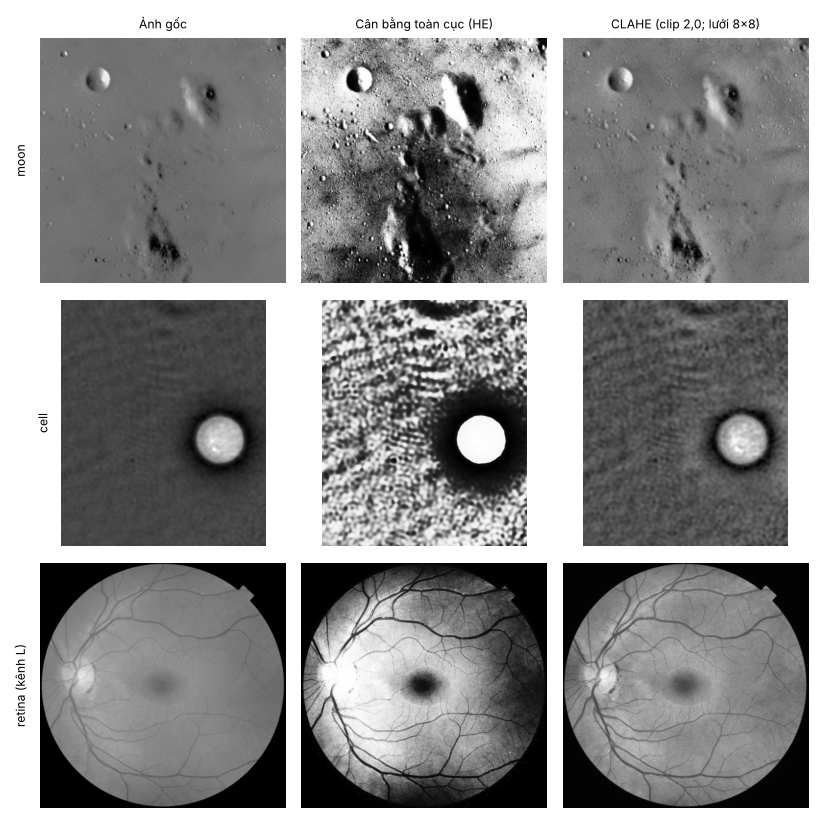
\includegraphics[width=0.78\textwidth]{w5_clahe.png}
\caption{Cân bằng lược đồ toàn cục (HE) và CLAHE. Hàng cuối là kênh $L$ của ảnh võng mạc.}
\label{fig:w5_clahe}
\end{figure}

\textbf{Ứng dụng.} CLAHE được dùng rộng rãi để tiền xử lý ảnh y khoa (X-quang, CT, ảnh đáy mắt), ảnh chụp dưới nước, ảnh thiếu sáng và ảnh sương mù, cũng như làm phép tăng cường dữ liệu.

% =====================================================================
\subsection{Vì sao cân bằng lược đồ phụ thuộc vào toàn bộ ảnh}
\label{subsec:w5_global}

\textit{Câu hỏi: Vì sao phương pháp cân bằng lược đồ (histogram equalization) thay đổi mức xám của ảnh không chỉ dựa trên giá trị mức xám tại mỗi điểm ảnh mà dựa trên toàn bộ ảnh?}

\textbf{Từ bài toán.} Cân bằng lược đồ tìm phép biến đổi đơn điệu tăng $T$ sao cho ảnh ra $g = T(f)$ có hàm mật độ \emph{đều}~\citep{xlav_lec3}. Theo công thức đổi biến của hàm mật độ (trang 27):
\begin{equation}
p_g(g) = \frac{p_f(f)}{|dT(f)/df|} = 1 \;\Rightarrow\; \frac{dT}{df} = p_f(f) \;\Rightarrow\; T(f) = \int_0^{f} p_f(w)\,dw,
\end{equation}
và trong trường hợp rời rạc $g_k = T(f_k) = \sum_{j=0}^{k} \frac{n_j}{n}$. Như vậy $T$ chính là \emph{hàm phân phối tích lũy} (CDF) của mức xám \emph{trên toàn ảnh}. Để biết $T(f_k)$, ta phải biết số điểm ảnh $n_j$ của mọi mức $j \le f_k$, tức phải duyệt toàn bộ ảnh.

\textbf{Ý nghĩa.} $T(f(x, y))$ là \emph{tỉ lệ điểm ảnh của cả ảnh có mức xám không lớn hơn $f(x, y)$}, tức thứ hạng (phân vị) của điểm ảnh trong toàn ảnh. Kết quả của một điểm phụ thuộc vào vị trí mức xám của nó so với tất cả các điểm còn lại, không chỉ vào giá trị của nó. Hệ số giãn tại mức $f$ là $dT/df = p_f(f)$: những khoảng mức xám có nhiều điểm ảnh được giãn nhiều, khoảng ít điểm ảnh bị nén. Đó là cách HE ``tự thích nghi'' với dữ liệu, khác với các ánh xạ ở Mục~\ref{subsec:w5_drawbacks} có hàm $T$ cố định.

\textbf{Ví dụ từ bài giảng} (trang 32, $n_G = 15$, $NM = 64$). Mức $f = 2$ có $H[2] = 16$ và $T[2] = H[0] + H[1] + H[2] = 0 + 4 + 16 = 20$, nên $T_R[2] = \mathrm{round}\big(\frac{14}{64} \cdot 20\big) = \mathrm{round}(4{,}375) = 4$. Nếu một ảnh khác cũng có điểm ảnh mức $2$ nhưng chỉ có $2$ điểm ảnh ở các mức $\le 2$, thì mức $2$ được ánh xạ thành $\mathrm{round}\big(\frac{14}{64} \cdot 2\big) = 0$. Cùng một giá trị mức xám nhưng cho kết quả khác nhau vì phân bố của toàn ảnh khác nhau.

\textbf{Lưu ý.} HE vẫn là \emph{phép toán điểm} theo nghĩa~(\ref{eq:w5_point_op}): hai điểm cùng mức xám luôn có cùng kết quả, và mỗi điểm được biến đổi qua một bảng tra. Điểm khác là \emph{bảng tra được xây dựng từ thống kê toàn cục} của ảnh. Hệ quả: (i) HE ``toàn cục'' không làm rõ được một vùng nhỏ nếu vùng đó chiếm ít điểm ảnh; (ii) các điểm cùng mức xám không thể tách ra, nên lược đồ kết quả chỉ \emph{gần} đều (lược đồ $H_g$ ở trang 34 có các cột $0$ xen kẽ các cột lớn). Muốn dùng thông tin cục bộ, ta chuyển sang AHE/CLAHE (Mục~\ref{subsec:w5_clahe}).

% =====================================================================
\subsection{Cài đặt đặc tả lược đồ dựa trên kỹ thuật cân bằng lược đồ}
\label{subsec:w5_hist_spec}

\textit{Câu hỏi: Sử dụng kỹ thuật cân bằng lược đồ để thực hiện đặc tả lược đồ (histogram specification) theo giải thuật ở trang 36--39 của bài giảng~\citep{xlav_lec3}. Viết chương trình cài đặt và chạy thử trên $10$ ảnh, hiển thị ảnh và lược đồ trước và sau khi biến đổi.}

\textbf{Ý tưởng.} Cho ảnh $f$ và một lược đồ mong muốn $p_g$. Đặt $s = T(f) = \int_0^f p_f$ là ánh xạ cân bằng lược đồ của $f$ và $z = G(g) = \int_0^g p_g$ là ánh xạ cân bằng lược đồ của lược đồ đích. Cả $s$ và $z$ đều có phân bố đều, nên có thể đồng nhất $z = s$, suy ra
\begin{equation}
g = G^{-1}(s) = G^{-1}\big(T(f)\big), \qquad F = G^{-1} \circ T.
\label{eq:w5_spec}
\end{equation}
Nói cách khác, ta \emph{cân bằng} ảnh $f$, rồi thực hiện \emph{phép ngược của phép cân bằng} của lược đồ đích. Kỹ thuật cân bằng lược đồ được dùng hai lần.

\textbf{Nghịch đảo rời rạc.} $G$ rời rạc là hàm đơn điệu tăng nhưng không nhất thiết tăng ngặt (khi $H_g[p] = 0$), nên ta định nghĩa $G^{-1}(s) = \min\{g : G[g] \ge s\}$ — mức xám nhỏ nhất có giá trị tích lũy đạt tới $s$. Do $G$ đơn điệu, phép tìm này dùng tìm kiếm nhị phân.

\begin{algorithm}[ht]
\caption{Đặc tả lược đồ dựa trên cân bằng lược đồ}
\label{alg:w5_spec}
\begin{algorithmic}[1]
\Require Ảnh xám $f$ kích thước $N \times M$, $n_G$ mức xám; lược đồ đích $p_g[0 \ldots n_G - 1]$, $\sum p_g = 1$
\Ensure Ảnh $g$ có lược đồ xấp xỉ $p_g$
\State $H_f[0 \ldots n_G - 1] \gets 0$; \quad \textbf{for} mỗi $(x, y)$: $H_f[f(x, y)] \gets H_f[f(x, y)] + 1$ \Comment{Bước 1--2}
\State $T[0] \gets H_f[0]$; \quad $T[p] \gets T[p - 1] + H_f[p]$, $p = 1, \ldots, n_G - 1$ \Comment{Bước 3}
\State $T[p] \gets \mathrm{round}\big(\frac{n_G - 1}{NM}\,T[p]\big)$ \Comment{Bước 4: bảng tra cân bằng của $f$}
\State $H_g[p] \gets NM \cdot p_g[p]$; \quad $G[0] \gets H_g[0]$; \quad $G[p] \gets G[p - 1] + H_g[p]$ \Comment{Bước 5}
\State $G[p] \gets \mathrm{round}\big(\frac{n_G - 1}{NM}\,G[p]\big)$ \Comment{Bước 6: bảng tra cân bằng của lược đồ đích}
\For{$s = 0, \ldots, n_G - 1$}
    \State $G^{-1}[s] \gets \min\{q : G[q] \ge s\}$ \Comment{tìm kiếm nhị phân}
\EndFor
\State $F[p] \gets G^{-1}[T[p]]$, $p = 0, \ldots, n_G - 1$ \Comment{bảng tra tổng hợp $F = G^{-1} \circ T$}
\State \textbf{for} mỗi $(x, y)$: $g(x, y) \gets F[f(x, y)]$ \Comment{Bước 7}
\State \Return $g$
\end{algorithmic}
\end{algorithm}

\textbf{Chương trình.} Chương trình được viết bằng Python (NumPy, OpenCV), chỉ dùng thư viện để đọc ảnh và đổi không gian màu; các bước cân bằng và đặc tả được cài đặt theo đúng giải thuật trên. Mã nguồn đầy đủ (kèm phần vẽ hình) nằm trong tệp \texttt{XLAV/code/w5\_histspec.py}. Phần cốt lõi:
\begin{lstlisting}[language=Python]
import numpy as np, cv2
nG = 256

def histogram(f):
    H = np.zeros(nG, np.int64)
    np.add.at(H, f.ravel(), 1)                       # Step 2: H[f(x,y)] += 1
    return H

def equalize_lut(H, NM):
    T = np.cumsum(H)                                 # Step 3: cumulative histogram
    return np.round((nG - 1) / NM * T).astype(np.int64)   # Step 4

def specify(f, pg):
    """g = G^{-1}[T[f]]; f: uint8 grey image, pg: target pdf (sum = 1)."""
    NM = f.size
    T = equalize_lut(histogram(f), NM)               # Steps 1-4
    G = np.round((nG - 1) / NM * np.cumsum(pg * NM)).astype(np.int64)  # Steps 5-6
    Ginv = np.searchsorted(G, np.arange(nG), side='left').clip(0, nG - 1)
    lut = Ginv[T]                                    # F = G^{-1} o T
    return lut[f].astype(np.uint8), lut              # Step 7

def apply_color(img, fn):
    """Colour image: transform only the V channel of HSV, keep H and S."""
    hsv = cv2.cvtColor(img, cv2.COLOR_RGB2HSV)
    hsv[..., 2] = fn(hsv[..., 2])
    return cv2.cvtColor(hsv, cv2.COLOR_HSV2RGB)

# predefined target histogram: Gaussian N(128, 45^2) on [0, 255]
z = np.arange(nG)
pg = np.exp(-(z - 128) ** 2 / (2 * 45.0 ** 2)); pg /= pg.sum()
\end{lstlisting}

\textbf{Thiết lập thực nghiệm.} Lược đồ đích được chọn là phân bố chuẩn $\mathcal{N}(128, 45^2)$ cắt trên $[0, 255]$: ảnh kết quả có độ sáng trung bình ở giữa thang xám, phần lớn điểm ảnh nằm trong khoảng $[38, 218]$, tránh bão hòa ở hai đầu như khi cân bằng về lược đồ đều. Mười ảnh thử lấy từ bộ ảnh chuẩn của thư viện \texttt{scikit-image}: $6$ ảnh xám (\texttt{camera}, \texttt{moon}, \texttt{coins}, \texttt{clock}, \texttt{cell}, \texttt{page}) và $4$ ảnh màu (\texttt{astronaut}, \texttt{coffee}, \texttt{chelsea}, \texttt{rocket}). Với ảnh màu, phép biến đổi chỉ áp dụng trên kênh $V$ của HSV. Để so sánh, mỗi ảnh được xử lý bằng cả cân bằng lược đồ (HE) và đặc tả lược đồ (HS). Kết quả ở Hình~\ref{fig:w5_spec1}, \ref{fig:w5_spec2} và Bảng~\ref{tab:w5_spec_stats}.

\begin{figure}[p]
\centering
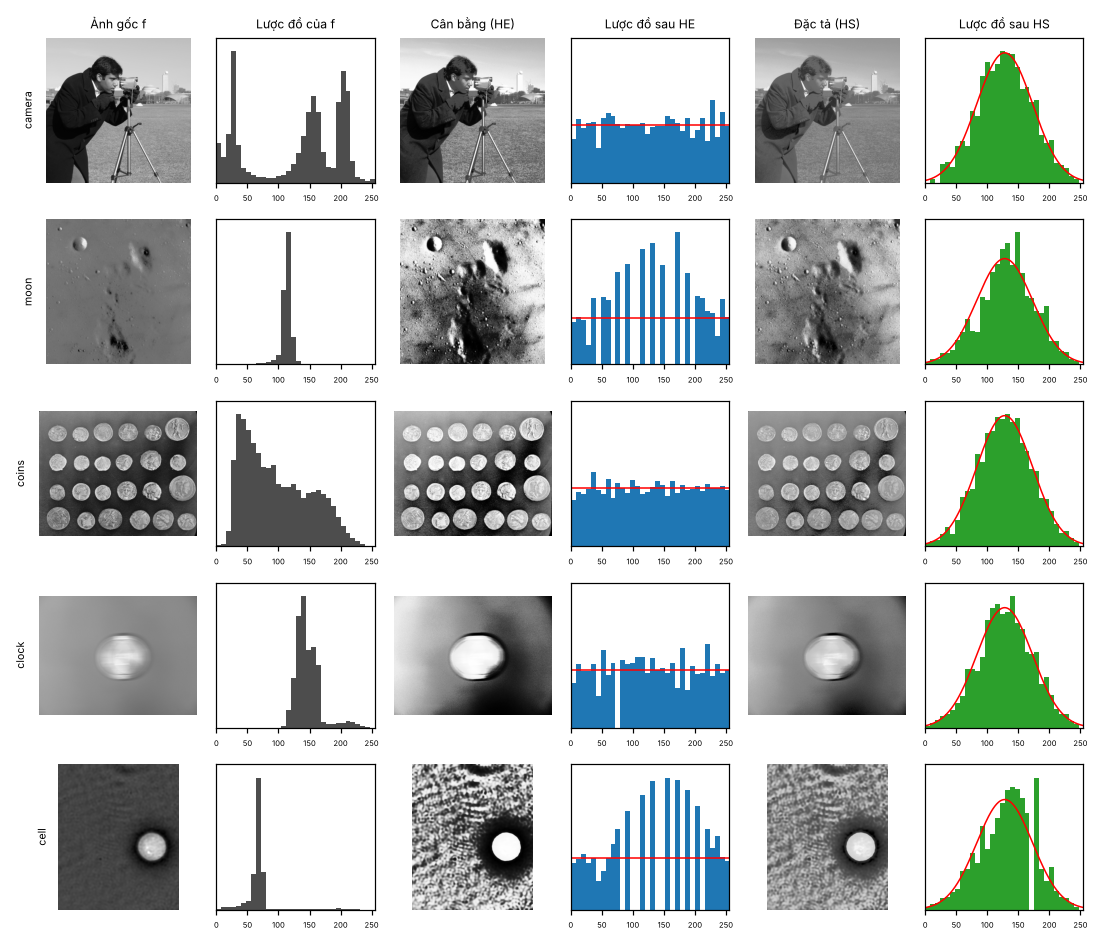
\includegraphics[width=\textwidth]{w5_histspec_1.png}
\caption{Đặc tả lược đồ trên $5$ ảnh xám đầu. Cột $2$, $4$, $6$: lược đồ (gộp $8$ mức/cột để dễ quan sát); đường đỏ ở cột $4$ là lược đồ đều, ở cột $6$ là lược đồ đích $\mathcal{N}(128, 45^2)$.}
\label{fig:w5_spec1}
\end{figure}

\begin{figure}[p]
\centering
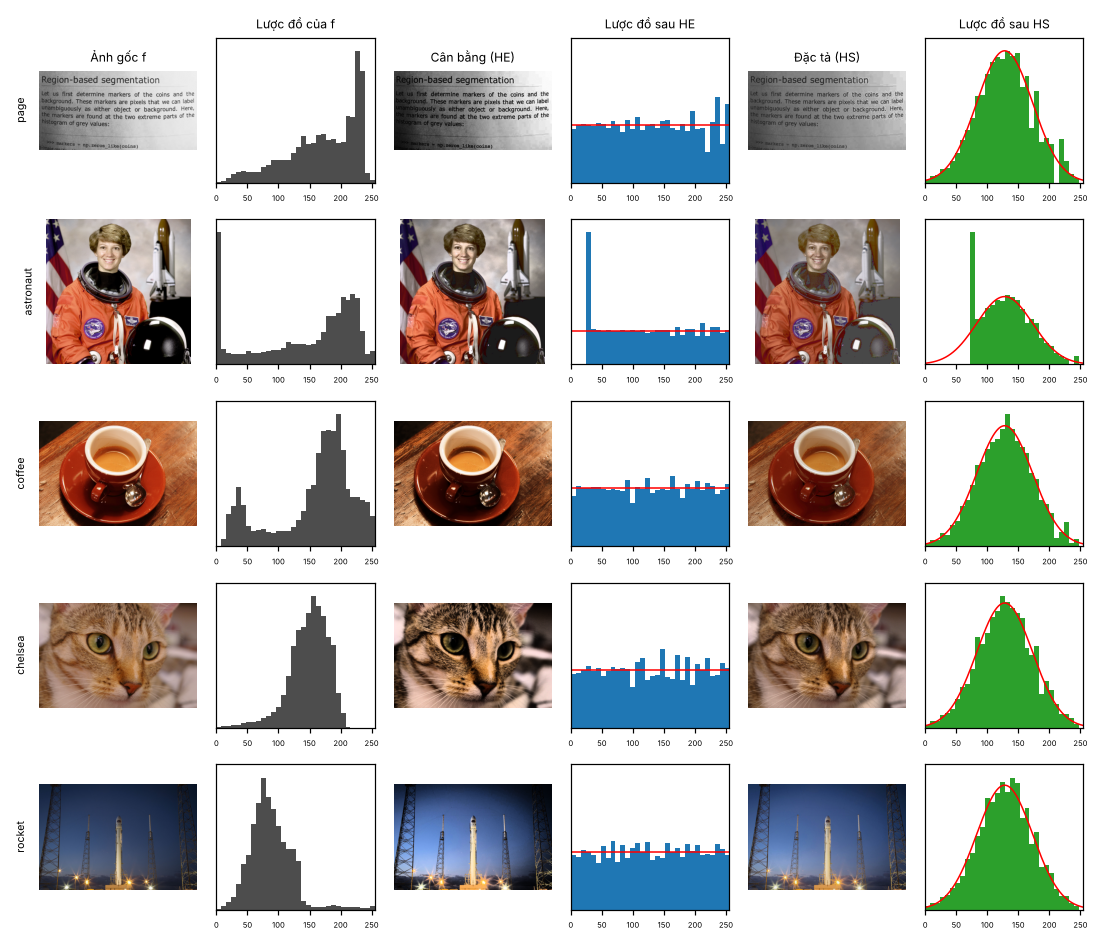
\includegraphics[width=\textwidth]{w5_histspec_2.png}
\caption{Đặc tả lược đồ trên ảnh \texttt{page} và $4$ ảnh màu (xử lý trên kênh $V$; lược đồ vẽ cho kênh $V$).}
\label{fig:w5_spec2}
\end{figure}

\begin{table}[ht]
\centering
\small
\caption{Trung bình và độ lệch chuẩn mức xám (kênh $V$ với ảnh màu) trước và sau biến đổi}
\label{tab:w5_spec_stats}
\renewcommand{\arraystretch}{1.15}
\begin{tabular}{|l|c|c|c|}
\hline
\textbf{Ảnh} & \textbf{Ảnh gốc $f$} & \textbf{Sau HE} & \textbf{Sau HS (đích $128 / 45$)} \\
\hline
camera & $129{,}1 / 73{,}6$ & $128{,}6 / 73{,}7$ & $128{,}4 / 43{,}9$ \\
moon & $112{,}2 / 13{,}3$ & $133{,}9 / 73{,}9$ & $131{,}0 / 44{,}5$ \\
coins & $96{,}9 / 52{,}9$ & $128{,}3 / 73{,}3$ & $128{,}1 / 43{,}8$ \\
clock & $146{,}3 / 20{,}9$ & $130{,}1 / 73{,}1$ & $129{,}0 / 43{,}7$ \\
cell & $68{,}0 / 23{,}9$ & $133{,}5 / 74{,}5$ & $130{,}9 / 44{,}7$ \\
page & $171{,}5 / 56{,}8$ & $128{,}5 / 74{,}3$ & $128{,}4 / 44{,}9$ \\
astronaut & $143{,}0 / 81{,}3$ & $129{,}6 / 71{,}8$ & $130{,}2 / 40{,}6$ \\
coffee & $158{,}6 / 63{,}0$ & $128{,}3 / 73{,}8$ & $128{,}1 / 44{,}3$ \\
chelsea & $147{,}7 / 32{,}2$ & $128{,}8 / 73{,}8$ & $128{,}3 / 44{,}3$ \\
rocket & $87{,}6 / 34{,}2$ & $128{,}8 / 73{,}5$ & $128{,}3 / 44{,}0$ \\
\hline
\end{tabular}
\end{table}

\textbf{Nhận xét.}
\begin{itemize}
    \item \textbf{Đúng mục tiêu.} Dù ảnh gốc rất khác nhau (tối như \texttt{cell}, sáng như \texttt{page}, tương phản rất thấp như \texttt{moon} với $\sigma = 13{,}3$), sau đặc tả mọi ảnh đều có trung bình $\approx 128$ và độ lệch chuẩn $\approx 44$, rất gần lược đồ đích ($128$, $45$). Lược đồ sau HS bám sát đường cong đích ở Hình~\ref{fig:w5_spec1}, \ref{fig:w5_spec2}. Đây là lợi ích chính của đặc tả lược đồ: \emph{chuẩn hóa} nhiều ảnh về cùng một phân bố.
    \item \textbf{So với HE.} HE luôn đưa $\sigma$ lên khoảng $73$--$74$ (gần $\sigma$ của phân bố đều trên $[0, 255]$, là $255/\sqrt{12} \approx 73{,}6$). Với các ảnh vốn có độ tương phản thấp (\texttt{moon}, \texttt{cell}, \texttt{clock}) kết quả HE bị gắt, nhiễu nền bị khuếch đại. HS với lược đồ đích hình chuông cho ảnh tự nhiên hơn, ít bão hòa ở hai đầu thang xám. HE chính là trường hợp riêng của HS khi $p_g$ là phân bố đều ($G$ là ánh xạ đồng nhất).
    \item \textbf{Giới hạn của phép toán điểm.} Ảnh \texttt{astronaut} có khoảng $10{,}7\%$ điểm ảnh ở mức $V = 0$ (nền đen, mũ bảo hiểm). Mọi điểm cùng mức xám phải có cùng kết quả, nên khối điểm này không thể bị ``tách'' ra để phủ phần đuôi trái của lược đồ đích: lược đồ sau HS có một cột cao tại mức $\approx 72$ và trống ở dưới mức đó, $\sigma$ chỉ đạt $40{,}6$. Tương tự, $98\%$ điểm ảnh của \texttt{moon} chỉ nằm trong khoảng $[58, 141]$ (khoảng $84$ mức xám); khi các mức này được trải ra trên $256$ mức đầu ra, mỗi mức vào chỉ chiếm một mức ra nên lược đồ kết quả có dạng răng lược. Đặc tả lược đồ rời rạc chỉ cho kết quả \emph{xấp xỉ}; muốn khớp chính xác phải phá vỡ các điểm cùng mức (ví dụ sắp thứ tự theo trung bình lân cận).
    \item \textbf{Ảnh màu.} Biến đổi trên kênh $V$ giữ nguyên sắc độ ($H$) và độ bão hòa ($S$): ảnh \texttt{coffee}, \texttt{chelsea} chỉ thay đổi độ sáng, không bị lệch màu như khi biến đổi riêng rẽ ba kênh $R$, $G$, $B$.
\end{itemize}

% =====================================================================
\subsection{Bảng so sánh các phương pháp biến đổi màu sắc}
\label{subsec:w5_table}

\textit{Câu hỏi: Lập bảng so sánh các phương pháp biến đổi màu sắc theo các tiêu chí: tên phương pháp, nguyên lý, phương pháp thực hiện, khả năng thay đổi chất lượng màu, hạn chế và hướng phát triển.}

Bảng~\ref{tab:w5_compare} tổng hợp các phương pháp của Bài giảng 3~\citep{xlav_lec3}, bổ sung phép biến đổi gamma và CLAHE (Mục~\ref{subsec:w5_clahe}). Trong bảng, ``hệ số giãn'' là đạo hàm $T'(f)$ của hàm ánh xạ (Mục~\ref{subsec:w5_log_exp_proof}).

\begin{table}[!htbp]
\centering
\scriptsize
\caption{So sánh các phương pháp biến đổi màu sắc (ánh xạ mức xám)}
\label{tab:w5_compare}
\renewcommand{\arraystretch}{1.3}
\begin{tabularx}{\textwidth}{|p{1.45cm}|p{2.2cm}|p{2.35cm}|X|X|X|}
\hline
\textbf{Phương pháp} & \textbf{Nguyên lý} & \textbf{Thực hiện} & \textbf{Khả năng thay đổi chất lượng màu} & \textbf{Hạn chế} & \textbf{Hướng phát triển} \\
\hline
Tuyến tính (độ sáng, độ tương phản) & Biến đổi mức xám tại mỗi điểm theo một hàm bậc nhất cố định; hệ số giãn $a$ như nhau trên toàn thang xám & $g = f + b$ (độ sáng), $g = a f$ (tương phản), $g = a f + b$; cắt về $[0, n_G - 1]$ & Làm sáng/tối toàn ảnh; tăng ($a > 1$) hoặc giảm ($a < 1$) độ tương phản đồng đều; tạo ảnh âm bản ($a = -1$) & Không phân biệt vùng tối, sáng; bão hòa và mất chi tiết khi $a$ lớn; tham số chọn thủ công & Chọn $a$, $b$ tự động theo thống kê ảnh (trung bình, độ lệch chuẩn); ánh xạ từng đoạn \\
\hline
Ánh xạ khoảng $[f_1, f_2] \to [g_1, g_2]$ & Đưa khoảng mức xám quan tâm lên khoảng mới, giữ vị trí tương đối & $g = \frac{g_2 - g_1}{f_2 - f_1}(f - f_1) + g_1$; ngoài khoảng thì cắt về $g_1$, $g_2$ & Kéo giãn tương phản tối đa cho khoảng quan tâm (cửa sổ hóa ảnh CT); tận dụng toàn bộ khoảng động & Mất thông tin ngoài $[f_1, f_2]$; nhạy với điểm ngoại lai khi lấy $[f_{\min}, f_{\max}]$ & Chọn $f_1$, $f_2$ theo phân vị; ánh xạ nhiều đoạn; cửa sổ hóa tương tác \\
\hline
Logarit & Hàm lõm, hệ số giãn $c/f$ giảm dần: giãn vùng tối, nén vùng sáng & $g = c \log(1 + f)$, $c = \frac{n_G - 1}{\log n_G}$ & Làm rõ chi tiết vùng tối, nén khoảng động lớn (phổ Fourier, ảnh HDR) & Đường cong cố định; làm ảnh sáng bị bạc; $\log 0$ không xác định & Biến đổi gamma $g = (n_G - 1)(f/(n_G - 1))^{\gamma}$ với $\gamma$ điều chỉnh được; ánh xạ tông màu (tone mapping) cục bộ \\
\hline
Mũ & Hàm lồi, hệ số giãn $e^{f}$ tăng dần: nén vùng tối, giãn vùng sáng & $g = e^{f}$; thực tế $g = (n_G - 1)\frac{e^{k f/(n_G - 1)} - 1}{e^k - 1}$ & Làm rõ chi tiết vùng sáng của ảnh dư sáng & Tràn số, phải chuẩn hóa; làm ảnh tối thêm tối; thêm tham số $k$ & Như trên (gamma $\gamma > 1$); kết hợp với phân đoạn vùng sáng \\
\hline
Cân bằng lược đồ (HE) & Tìm $T$ để ảnh ra có hàm mật độ đều; $T$ là CDF của ảnh, hệ số giãn $T' = p_f$ & $C[p] = \sum_{j \le p} H[j]$; \newline $T[p] = \mathrm{round}\big(\frac{n_G - 1}{NM}C[p]\big)$; \newline $g = T[f]$ & Tự động, không cần tham số; tăng mạnh độ tương phản của ảnh có lược đồ tập trung & Khuếch đại nhiễu ở vùng đồng nhất; ảnh gắt, không tự nhiên; lược đồ chỉ gần đều; toàn cục, không làm rõ vùng nhỏ & AHE, CLAHE; HE bảo toàn độ sáng (BBHE, DSIHE); áp dụng trên kênh độ sáng cho ảnh màu \\
\hline
Đặc tả lược đồ (HS) & Biến đổi để ảnh ra có lược đồ cho trước; dùng HE hai lần & $g = G^{-1}[T[f]]$ (Giải thuật~\ref{alg:w5_spec}) & Chuẩn hóa nhiều ảnh về cùng phân bố; chuyển phong cách màu theo ảnh mẫu; kiểm soát được kết quả & Phải chọn lược đồ đích phù hợp; không tách được các điểm cùng mức xám; vẫn là phép toán điểm & Đặc tả chính xác (phá vỡ các điểm cùng mức); đặc tả lược đồ màu nhiều chiều; chuyển màu bằng học sâu \\
\hline
CLAHE (bổ sung) & HE cục bộ theo từng ô, cắt lược đồ để chặn hệ số giãn & Giải thuật~\ref{alg:w5_clahe}: lược đồ từng ô, cắt theo $\alpha$, nội suy song tuyến giữa các ô & Làm rõ chi tiết cục bộ ở cả vùng tối và vùng sáng; hạn chế khuếch đại nhiễu & Hai tham số (lưới, hệ số cắt); có thể tạo quầng sáng quanh biên; tốn tính toán hơn HE & Tự chọn tham số theo nội dung ảnh; kết hợp khử nhiễu; tăng cường ảnh thiếu sáng bằng học sâu \\
\hline
\end{tabularx}
\end{table}
